\documentclass{article}

\usepackage{mathrsfs,amsmath}
\usepackage{xcolor}
\usepackage{titlesec}
\usepackage{listings}
\usepackage{syntax}
\usepackage{pythonhighlighting}
\usepackage{fancyvrb}

\usepackage{graphicx}

\graphicspath{ {./assets/} }

\usepackage[margin=1.4in]{geometry}

\title{Homework \#3 | Fall 2021} 
\author{Jared Dyreson\\ 
        California State University, Fullerton}

\DeclareRobustCommand{\bowtie}{%
  \mathrel\triangleright\joinrel\mathrel\triangleleft}


\usepackage [english]{babel}
\usepackage [autostyle, english = american]{csquotes}
\MakeOuterQuote{"}

\titlespacing*{\section}
{0pt}{5.5ex plus 1ex minus .2ex}{4.3ex plus .2ex}
\titlespacing*{\subsection}
{0pt}{5.5ex plus 1ex minus .2ex}{4.3ex plus .2ex}

\usepackage{hyperref}
\hypersetup{
    colorlinks,
    citecolor=black,
    filecolor=black,
    linkcolor=black,
    urlcolor=black
}

\begin{document}

\maketitle
\tableofcontents

\newpage


\section{Questions}

\subsection{Offline Ski Rental}

\subsubsection{Problem Description}

\begin{table}[!h]
\begin{tabular}{|l|l|}
\hline
\textbf{input} & a daily ski rental price $r > 0$, purchase price $p > 0$, and number of days $d > 0$ \\ \hline
\textbf{output} & \begin{tabular}[c]{@{}l@{}}True if it is cheaper to rent skis for d days at r dollars per day, or False if it is\\ cheaper to buy skis for p dollars\end{tabular} \\ \hline
\end{tabular}
\end{table}

\subsubsection{Pseudocode}

\begin{verbatim}
function ski(int rate, int purchasePrice, int days):
    rental_total = rate * days
    return rental_total < purchasePrice
\end{verbatim}

\subsubsection{Time Complexity}

This function is quite simple, as we are given all the information up front.
Each operation we have will complete in a time complexity of $O(1)$.
Therefore, the best/worst case of this is $O(1)$.

\subsubsection{Implementation}

\begin{python}

def solution(rental_price: int,
             purchase_price: int, days: int) -> bool:

    return (rental_price * days) < purchase_price
\end{python}

\newpage

\subsection{List Reversal}

\subsubsection{Problem Description}

\begin{table}[!h]
\begin{tabular}{|l|l|}
\hline
\textbf{input} & a list L of n elements \\ \hline
\textbf{output} & a list containing the elements of L but in reversed order \\ \hline
\end{tabular}
\end{table}

\subsubsection{Pseudocode}

\begin{verbatim}
function reverse(container):
    last_index = container.length # O(1)
    for element in container: # O(n)
        swap(element, container[last_index]) # O(1)
        last_index = last_index - 1 # O(1)
    return container # O(1)
\end{verbatim}

\subsubsection{Time Complexity}

This function will modify the container in place and does not create a copy.
Other variants can leave the original container intact and return a reversed copy.
The benefit of this would be data integrity, however, that is at the expense of having to have duplicate data.
We need to iterate over the entire container of "n" elements and we assume the swap function is of constant time.
Therefore, time complexity of this function is linear, or $O(n)$.
\subsubsection{Implementation}

\begin{python}
def solution(container: list) -> list:
    end = len(container) - 1
    for x, _ in enumerate(container):
        if x < end:
            container[x], container[end] = container[end], container[x]
            end -= 1
    return container
\end{python}

\newpage

\subsection{Pythagorean Triple}

\subsubsection{Problem Description}
\begin{table}[!h]
\begin{tabular}{|l|l|}
\hline
\textbf{input} & two positive integers; $a$ and $b$ with $a < b$ \\ \hline
\textbf{output} & \begin{tabular}[c]{@{}l@{}}a Pythagorean triple (x, y, z), such that $x$, $y$, and $z$ are positive integers,\\ $a \le x \le y \le z \le b$ and $x^{2} + y^{2} = z^{2}$, or None if no such triples exist\end{tabular}\\ \hline
\end{tabular}
\end{table}

\subsubsection{Pseudocode}

\begin{verbatim}
function validator(tuple[int, int, int] triplet):
    x, y, z = triplet # O(3), assignment and unpacking for three elements
    return z == square_root(x ** 2 + y ** 2) and x <= y <= z
    # O(n) <- for the squaring of x and y. This is building off the previous
    # assumption made in Project 2 for the Fibonacci sequence

function pythagorean_triples(int a /* lower bound */, int b /* upper bound */):
    candidates = [] # O(1)
    for x in range(a, b + 1): # get range of values, bounded by a and b # O(n)
        candidates.append(x) # O(1)
    # create all permutations
    # description does not specifically instruct to create an algorithm
    # to create these permutations, therefore we use the best case
    # of O(n^r), where r represents the length of the tuple -> O(n^3)
    permutations = generate_permutations(iterable=candidates, r=3) # O(n^3)
    # this is the function signature of itertools.combinations
    valid_triplets = [] # O(1)

    # this for loop block runs in O(n^2)
    for permuation in permutations: # O(n)
        if(validator(permuation)): # O(n)
            valid_triplets.append(permutation) # O(1)
    return valid_triplets # O(1)
\end{verbatim}

\subsubsection{Time Complexity}

The main portion of this algorithm comes solely from creating all possible combinations the range presents.
Here, we are tasked with creating triplets, given a range of numbers $a$ and $b$.
The creation of all possible combinations will take $O(n^{r})$, where $r$ is the length of the container you're producing.
Therefore in our case it is $O(n^{3})$ and more information regarding this can be found in \href{https://stackoverflow.com/a/20765011}{\underline{this StackOverflow comment thread}}.
All of these triplets need to then be processed by our validator function, which was defined in the problem description.
These validations will occur in $O(n)$ time, because we are assuming raising a number to a given power will take that time complexity.
It is disputed in implementations in Python, either $O(1)$ or $O(n)$ and since a previous homework assignment uses the latter, we will go with this assumption.
Overall, the time complexity will be of $O(n^{3})$, as it the leading term in the polynomial $O(n^{3}) + O(n^{2})$.


\newpage

\subsubsection{Implementation}

\begin{python}
import itertools
import math

def validator(container: tuple[int, int, int]) -> bool:
    x, y, z = container  # raise ValueError if container len != 3
    # x ^ 2 + y ^ 2 = z ^ 2
    # where x, y and z are perfect squares
    return z == math.sqrt(x ** 2 + y ** 2) and x <= y <= z

def solution(integers: tuple[int, int]) -> list[tuple[int, int, int]]:
    a, b = integers  # a is lower bound and b is upper bound
    if not(isinstance(a, int)
           and isinstance(b, int)
           and a < b):
        raise ValueError(
            f'[ERROR] Expected integers for `a` ({a}) and `b` ({b}), where a < b')
    candidates = [_ for _ in range(a, b+1)]
    """
    Given a = 1 and b = 4
    - (1, 2, 3)
    - (2, 3, 4)
    are all valid combinations
    """

    return [candidate for candidate in
            itertools.combinations(candidates, 3) if validator(candidate)]
\end{python}


\newpage

\subsection{Missing Integer}

\subsubsection{Problem Description}

\begin{table}[!h]
\begin{tabular}{|l|l|}
\hline
\textbf{input} & \begin{tabular}[c]{@{}l@{}}an array $A$ of size $N-1$ that contains all integers in the range of $1$ to $N$,\\ except one missing integer. This list contains no duplicates.\end{tabular} \\ \hline
\textbf{output} & the missing number from the list \\ \hline
\end{tabular}
\end{table}

\subsubsection{Pseudocode}

\begin{verbatim}
function missing_element(container: list[int]):
    N = len(container) + 1
    intended_sum = N * (N + 1) / 2 # Gaussian Sum
    return intended_sum - sum(container) 
    # the missing element is the difference between each container
\end{verbatim}


\subsubsection{Time Complexity}

This function is quite efficient in finding the missing integer, as it only needs to loop through the container once.
Also, the algorithm does not require the list to be in sorted order and can be extended to tuples, sets and other Python data containers.
First, we need to compute the Gaussian Sum of the container as if it was intact.
The formula for this is:
$$\frac{N \times (N + 1)}{2}$$
and assumes the sequence is monotonically increasing, and contains all integers from $1$ to $N$ inclusive.
Here, we have access to a key characteristic of the container without having to reconstruct it.
Then, we translate the current container in terms of an integer and we apply the sum function $O(n)$.
Subtracting the difference between the two will give you the missing integer.
This will  run in $O(n)$ time, as the only linear aspect is to find the sum of the current container.
\subsubsection{Implementation}

\begin{python}
def missing_integer(container: typing.List[int], dialation: int = 1) -> int:
    """
    Find the missing integer in a monotonically increasing sequence
    """

    intended_sum = gaussian_sum(len(container) + 1)

    return intended_sum - sum(container)


def gaussian_sum(N: int, dialation: int = 1) -> int:
    """
    This is the sum of a contiguous sequence of integers
    Dialation is applied when a constant is applied to all elements in the sequence
    """

    return int(N * (N + 1) / 2) * dialation
\end{python}


\newpage

\section{Extra Credit}

\subsection{Street Map}

\begin{figure}[!h]
\centering
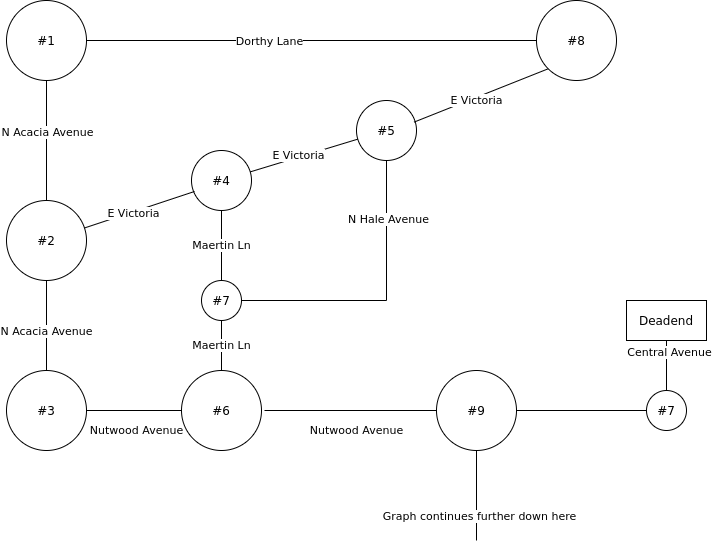
\includegraphics[width=10cm]{StreetMap}
\caption{Street View of Troy High School backroads}
\end{figure}

Each node can contain the following information, and applying this to node \#1 we get:

\begin{itemize}
\item Lateral intersection | Dorthy Lane (East/West)
\item Medial intersection | Acacia Avenue (South/North)
\item Longitude | SomeValue
\item Latitude | SomeValue
\item Dead end | False
\end{itemize}

Each edge on the graph represents the street connecting each intersection and each edge is bidirectional (forgot to make it so in the diagram).

\newpage

\subsection{Course Requirements}

\begin{figure}[!h]
\centering
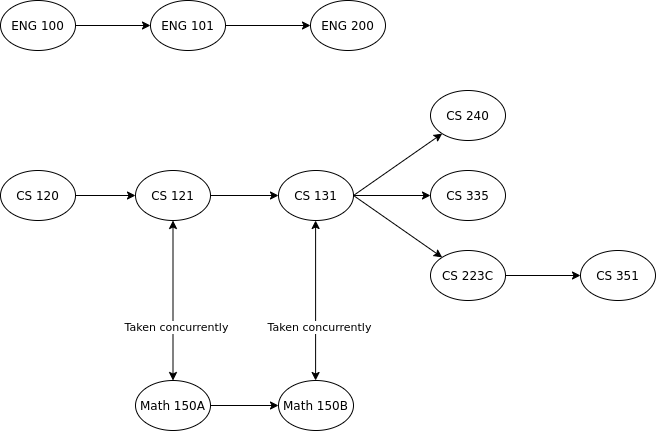
\includegraphics[width=10cm]{CourseRequirements}
\caption{Example set of courses to be taken}
\end{figure}

Each class should be taken in sequential order and must have it's prerequisites met before.
This is called a topological graph and is applied in different areas such as package managers and neuroscience.
As shown here in this example, some sections or "forests" can exist independently of one another.
These do not have interlaced dependencies and can be completed in their own continuum.
Others are connected on a basis where the course  must be taken in conjunction with the another class.
This can be seen in CS 121 and Math 150A, however this can also be applied to lab courses and their associated lecture (PHYS 225 and PHYS 225L).

\newpage

\subsection{Social Media Network}

\begin{figure}[!h]
\centering
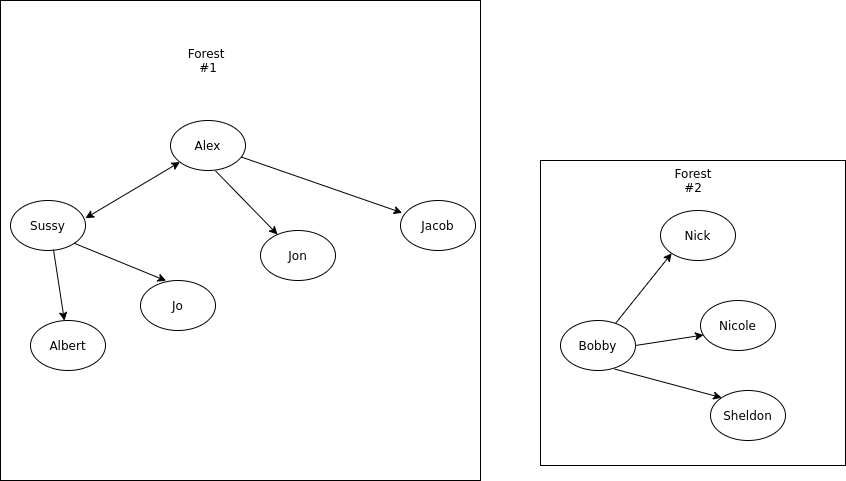
\includegraphics[width=13cm]{SocialMediaNetwork}
\caption{Example Social Media Network}
\end{figure}

Given the list of people and their associated friends, we can construct a graph showing their relationships.
\begin{itemize}
\item Sussy $\rightarrow$ Alex, Jo, Albert
\item Alex $\rightarrow$ Jacob, Sussy, Jon
\item Bobby $\rightarrow$ Nick, Nicole, Sheldon
\end{itemize}

Singly directed edges can be read as "Person 1 is following Person 2 but Person 2 is not following Person 1".
Bidirectional edges are when both parties are following each other.
Each "forest" is a collection of  nodes where they are all connected in some fashion.
The separation occurs when there are not mutual connections between every element in the network

\end{document}
